\documentclass[11pt]{article}
\usepackage[margin=.79in]{geometry}
\PassOptionsToPackage{cmex10}{amsmath}
\usepackage{amssymb,amsmath,booktabs,graphicx,hyperref}
\hypersetup{colorlinks=true,urlcolor=blue,linkcolor=black}
\graphicspath{{figures/}{../docs/figures/}}
\title{The Throughput Cost of Smoothing GPU Timings\\in Speculative Decoding}
\author{Angelina Quan \qquad MIT 18.657}
\date{November 23, 2026}
\newtheorem{proposition}{Proposition}
\newtheorem{theorem}[proposition]{Theorem}
\newenvironment{proof}{\par\noindent\textit{Proof.}\ }{\unskip\nobreak\hfill$\square$\par}
\begin{document}
\DeclareFontShape{OMX}{cmex}{m}{n}{<->cmex10}{}
\maketitle
\begin{abstract}
In speculative decoding, a draft model proposes tokens and a target model checks them together. How many tokens should the target check in one pass? The DSpark scheduler in vLLM answers using two estimates: how many proposed tokens will be accepted and how long verification will take. It measures GPU time at several input sizes, then replaces each measurement with the largest time seen at that size or below. This can hide a useful feature of the hardware: a larger input sometimes runs faster than a smaller one. We test a single change to the scheduler: use the median time measured at each size directly. On one H200 serving Qwen3-4B with DSpark, this change increased warmed-up throughput from 6,059 to 6,251 output tokens per second on 768 held-out prompts at batch size 64, a gain of 3.17\% over the native scheduler (95\% paired bootstrap interval, 1.13--5.45\%). All outputs matched ordinary greedy decoding. A separate batch-32 study found a 1.35\% gain. At batch 64, the comparison with fixed widths chosen separately for each domain was inconclusive. The results show that how a scheduler summarizes GPU measurements can affect decoding speed even when its token predictions stay fixed.
\end{abstract}
\section{Why the timing table matters}
In speculative decoding, a drafter proposes several tokens and a target model verifies them in parallel~\cite{leviathan}. Checking a longer prefix can commit more tokens per target call. Its value depends on both the chance those tokens will be accepted and the cost of checking them. DSpark estimates prefix survival with a trained confidence head and allocates verification work across requests~\cite{dspark}. Two schedulers with identical predictions about the text can therefore make different decisions solely because they predict different GPU times.

The vLLM implementation profiles execution sizes and smooths the resulting table to suppress noisy decreases~\cite{native}. A running maximum has an asymmetric consequence. One slow measurement raises the estimated cost of every subsequent size until an even slower measurement appears. If a later size consistently executes faster, the scheduler cannot exploit that dip. Conversely, retaining every dip risks favoring a measurement that will disappear on the next engine launch. Which effect dominates is an empirical question.

\paragraph{Reading the interval on the time scale.} If $G=T_b/T_m-1$ is the fractional throughput gain, the fraction of baseline generation time saved at equal output count is $1-T_m/T_b=G/(1+G)$. Thus 3.17\% higher throughput corresponds to about 3.07\% less generation time. Applying the same increasing transformation to the paired interval gives approximately $[1.12,5.17]\%$ time saved. Averaging percentage gains for individual prompts would answer a different question and would ignore their shared execution within batches.

\clearpage
\section{Changing the verification-cost estimator}
For increasing captured sizes $n_1,\ldots,n_J$, let $m_j$ be the median profiled target-forward time at $n_j$. For a requested size $n$ within the captured range, let $j$ index the smallest captured size at least as large as $n$. The two estimates are
\[
 C_{\rm native}(n)=\max_{\ell\le j}m_\ell,\qquad C_{\rm measured}(n)=m_j .
\]
Both policies retain the same extrapolation beyond the capture limit, draft-cost estimates, pretrained confidence head, verifier, and allocation logic. Profiling precedes the timed runs. The intervention adds no per-step fitting.

The scheduler chooses a budget by weighing the expected number of committed tokens against estimated step time. A flat target-cost estimate can make a larger budget look effectively free. A measured curve with several distinct costs can give a smaller budget a higher expected throughput. The direction depends on the operating point.
\begin{figure}[h!]\centering
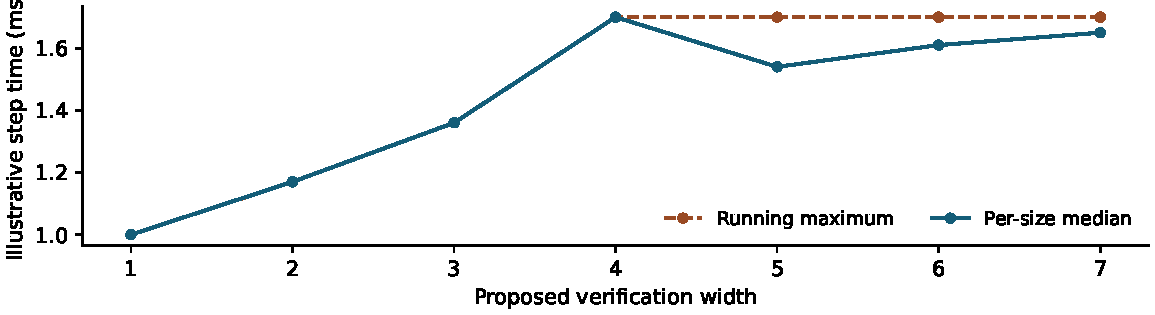
\includegraphics[width=.94\linewidth]{course_cost.pdf}
\caption{Worked example with hypothetical profile medians. The slow measurement at width four masks the faster measured sizes that follow. The held-out experiment appears in Figure~\ref{fig:confirm}.}
\end{figure}

\begin{figure}[h!]\centering
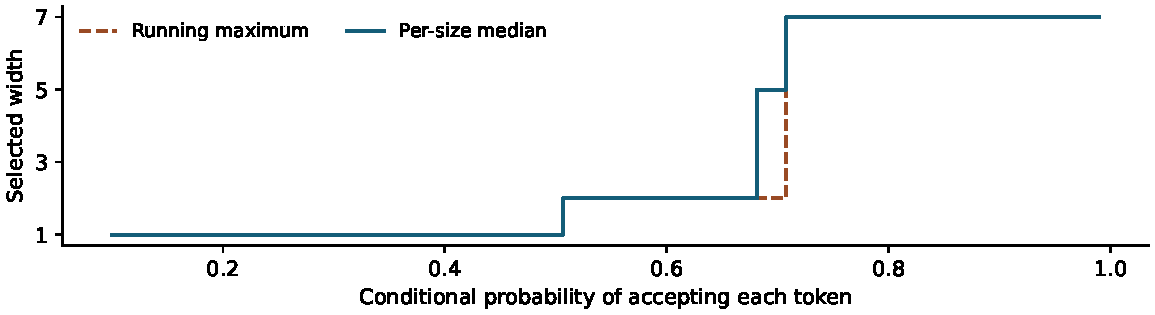
\includegraphics[width=.91\linewidth]{course_budget.pdf}
\caption{Using the hypothetical costs $C(w)$ above, choose the width maximizing $(1+\sum_{k=1}^w p^k)/C(w)$. Even when both policies see identical conditional acceptance probabilities $p$, their selected widths can differ. This simplified example illustrates the decision rule.}
\end{figure}
\clearpage
\section{From prefix probabilities to a budget decision}
Fix the batch state immediately before verification. For request $i$, let $L_i$ be the length of its accepted draft prefix and $s_{ik}=\Pr(L_i\geq k\mid\text{state})$. If request $i$ receives $w_i$ verification slots, the number of accepted drafts is $\min(L_i,w_i)$. The tail-sum identity gives
\begin{equation}
 \mathbb E[\min(L_i,w_i)\mid\text{state}]
 =\sum_{k=1}^{w_i}s_{ik}.
 \label{eq:survival}
\end{equation}
\begin{proposition}[Prefix allocation] At a fixed budget, choosing the largest prefix-survival probabilities, with ties broken in favor of earlier positions, maximizes expected accepted length.\end{proposition}
\begin{proof} Pointwise, $\min(L_i,w_i)=\sum_{k=1}^{w_i}\mathbf 1\{L_i\geq k\}$. Thus neither independence among tokens nor independence among requests is required. For a total budget $B$, write the idealized expected progress as
\begin{equation}
 R(B)=r_0+\max_{\substack{\sum_i w_i=B\\0\le w_i\le K}}
                 \sum_i\sum_{k=1}^{w_i}s_{ik},
 \qquad Q(B)=\frac{R(B)}{D(B)} ,
\end{equation}
where $r_0$ is the common base progress, $K$ is the draft cap and $D(B)>0$ is the full step cost. Each $s_{ik}$ is nonincreasing in $k$. Selecting the $B$ largest survival probabilities therefore attains the maximum: break ties in favor of earlier positions so that each selected slot includes its predecessors. \end{proof} This explains the scheduler's tradeoff while abstracting from implementation details.

\paragraph{The decision boundary.} For budgets $a<b$, define $\Delta R=R(b)-R(a)$ and $\Delta D=D(b)-D(a)$. Cross-multiplying the two positive denominators yields
\begin{equation}
 Q(b)>Q(a)\quad\Longleftrightarrow\quad
 \frac{\Delta R}{R(a)}>\frac{\Delta D}{D(a)}.
 \label{eq:boundary}
\end{equation}
The gain in expected tokens must exceed the relative increase in cost. Even when the predicted tokens are exactly the same under both schedulers, a change in the right-hand side can reverse the decision.

In Figures 1--2 take $p=0.70$. Widths 2 and 5 offer $R(2)=2.190$ and $R(5)=2.941$ expected tokens, a 34.3\% increase. Their measured example costs rise from 1.17 to 1.54 ms (31.6\%), whereas the envelope raises the latter to 1.70 ms (45.3\%). Equation~\eqref{eq:boundary} therefore favors width 5 under the measured table and width 2 under the envelope. These are also the respective maximizers over all seven candidate widths in the figure.

\clearpage
\section{When does a more precise profile help?}
Let $c_j$ denote the population median target time at captured size $j$ under a fixed profiling protocol. Write $m_j=c_j+e_j$ for its sample median and define the depth of the true timing dip by $d_j=\max_{\ell\le j}c_\ell-c_j$. Consider the event $\max_j|e_j|\le\epsilon$. \begin{proposition}[Distortion from the running maximum] On this event, the per-size median has strictly smaller absolute error at every size with $d_j>2\epsilon$.\end{proposition}
\begin{proof} We first bound both errors:
\begin{equation}
 |m_j-c_j|\le\epsilon,\qquad
 d_j-\epsilon\le \max_{\ell\le j}m_\ell-c_j\le d_j+\epsilon .
\end{equation}
For the upper bound apply $m_\ell\le c_\ell+\epsilon$ before taking the maximum. For the lower bound evaluate $m_\ell$ at a maximizer of $c_\ell$. Consequently, whenever $d_j>2\epsilon$, the measured estimate has strictly smaller absolute error at size $j$. \end{proof} With a finite grid and consistent sample medians, the envelope error converges to $d_j$. Repeated profiling alone cannot remove that distortion. This is a statement about the profiling distribution; medians from startup may themselves transfer poorly to generation.

\paragraph{From estimation error to decision loss.} Suppose for this calculation that the progress forecast is fixed and the estimated full step time $\widehat D(B)$ has relative error at most $\eta<1$ for every candidate budget. Let $B^*$ maximize $R(B)/D(B)$ and $\widehat B$ maximize $R(B)/\widehat D(B)$. \begin{proposition}[Budget selection under cost error] For $Q(B^*)>0$, the selected budget attains at least a fraction $(1-\eta)/(1+\eta)$ of the optimal one-step throughput.\end{proposition}
\begin{proof} By relative-error control and the definition of the estimated maximizer,
\begin{align}
 Q(\widehat B)
 &\ge (1-\eta)\frac{R(\widehat B)}{\widehat D(\widehat B)}
 \ge (1-\eta)\frac{R(B^*)}{\widehat D(B^*)}
 \ge \frac{1-\eta}{1+\eta} Q(B^*).
\end{align}
The first and last inequalities apply the relative-error bounds; the middle one uses optimality for the estimated table.\end{proof} In particular, if the ratio of the best true score to the runner-up exceeds $(1+\eta)/(1-\eta)$, the selected budget is stable. Close decisions can flip even with accurate profiling. The bound concerns a single batch state. The observed 3.17\% is a separate measurement over complete generations, whose subsequent states depend on earlier choices.

\paragraph{A testable implication.} In repeated profiles, record each budget's dip depth and variation across launches. On matched scheduler states, record the gap between the two highest predicted throughput scores. The analysis predicts a specific place to look for consequential disagreements: budgets with reproducible timing dips that compete closely under the native table. Timing both candidate budgets on those states would directly test the proposed mechanism.
\clearpage
\section{How many profile repetitions resolve a timing dip?}
The preceding propositions use a simultaneous error tolerance. To connect that tolerance to a profiling experiment, choose a time scale $h>0$ and an error probability $\delta\in(0,1)$ in advance.
\begin{theorem}[Finite-sample resolution of timing dips]
At each of $J$ sizes, take an odd number $n$ of independent, identically distributed timing measurements with median $c_j$. Suppose there exists $\gamma>0$ such that, at every size,
\[
 \Pr(X_j<c_j-h)\le\tfrac12-\gamma,\qquad
 \Pr(X_j>c_j+h)\le\tfrac12-\gamma .
\]
If $n\ge\log(2J/\delta)/(2\gamma^2)$, then with probability at least $1-\delta$ all sample medians lie within $h$ of their respective population medians. On this event the per-size median has strictly smaller absolute error than the running maximum at every size with $d_j>2h$.
\end{theorem}
\begin{proof}
Fix $j$. If the median exceeds $c_j+h$, then at least $(n+1)/2$ observations exceed $c_j+h$. Let $Z_i$ indicate such an exceedance. Since $\mathbb E Z_i\le 1/2-\gamma$, the sample average of these independent indicators must exceed its expectation by at least $\gamma$. Hoeffding's inequality~\cite{hoeffding} bounds this probability by $\exp(-2n\gamma^2)$. Applying the same argument to indicators of observations below $c_j-h$ bounds the lower tail. Taking a union bound over both tails and all sizes yields
\[
 \Pr\left(\max_{j\le J}|m_j-c_j|>h\right)
 \le 2J\exp(-2n\gamma^2)\le\delta .
\]
The last statement follows from Proposition 2 with $\epsilon=h$. Dependence between sizes is permitted by the union bound.
\end{proof}
\paragraph{Observable implication.} Define the empirical dip $\widehat d_j=\max_{\ell\le j} m_\ell-m_j$. On the simultaneous event, the running maximum and the final median are each within $h$ of their population counterparts, so $|\widehat d_j-d_j|\le2h$. Hence $\widehat d_j>4h$ certifies $d_j>2h$ and a strict reduction in cost-estimation error. This sufficient threshold may miss smaller useful dips.

\paragraph{Empirical scope.} Closely spaced timings may share thermal or load effects. The serving experiments did not estimate $\gamma$ or validate independence of within-size profiling repeats. The theorem guides the design of a repeated-profile experiment. The throughput interval below comes from paired serving measurements.
\clearpage
\section{Experimental design}
We ran Qwen3-4B with the released seven-token DSpark drafter using vLLM 0.33.0 on one H200. Greedy decoding used a 128-token output cap, a 2,048-token context limit, FP32 tensors, batch-invariant Triton attention, and disabled prefix caching. The experiment checked tokens against ordinary greedy decoding across every warmup and timed pass. The tensor setting alone does not establish the arithmetic precision of every kernel.

\begin{table}[h!]\centering\small
\begin{tabular}{lrr}\toprule
 & Batch 32 & Batch 64\\\midrule
Held-out prompts &384&768\\
Prompts per domain &128&256\\
Prompt batches per domain &4&4\\
Balanced engine orders &4&4\\
Warmup / timed passes per session &2 / 2&2 / 2\\
Global fixed width chosen before test &7&7\\\bottomrule
\end{tabular}
\caption{Two disjoint evaluations with equal representation from Alpaca (conversation), GSM8K (math), and MBPP (code). Each uses 16 engine sessions.}
\end{table}

Separate exploratory runs compared fixed widths 1 through 7 before the held-out comparisons. At batch 64 we also prespecified width 3 for chat and width 7 for math and code. This comparator uses known domain labels and combines the corresponding measured timings. It tests how much of the gain a simple domain-aware deployment could recover.

\paragraph{Estimand and uncertainty.} For equal output token counts, aggregate throughput gain is $100(T_b/T_m-1)$, where $T_b$ and $T_m$ are the baseline and measured-policy generation times summed across matched observations. Initialization and profiling are outside those times. We use 10,000 paired, domain-stratified batch-and-round bootstrap draws, resampling the same batches and rounds across methods and keeping repeated passes together. The intervals describe workload and timing variation within the tested setup. Each study has only four rounds and four prompt batches per domain.

\section{Results}
\begin{table}[h!]\centering\small
\begin{tabular}{rlrr}\toprule
Batch & Comparator & Throughput gain & 95\% interval\\\midrule
32 & Native adaptive & $+1.35\%$ & $[1.07,1.63]\%$\\
32 & Global fixed width & $+1.25\%$ & $[0.90,1.59]\%$\\
64 & Native adaptive & $+3.17\%$ & $[1.13,5.45]\%$\\
64 & Global fixed width & $+2.56\%$ & $[0.85,4.27]\%$\\
64 & Domain-specific widths & $+1.24\%$ & $[-1.20,3.94]\%$\\\bottomrule
\end{tabular}
\caption{Held-out throughput differences from retaining measured verification costs. Positive values favor the measured policy.}
\end{table}

At batch 64, throughput reaches 6,250.80 tokens/s, compared with 6,058.87 for native adaptive verification, 6,095.03 for global width 7, and 6,174.37 for the domain-specific policy. An earlier unbalanced exploratory run estimated a 4.98\% gain over native adaptive verification. The independent expansion yielded the smaller estimate in Table 2, below the original 5\% practical target.
\clearpage
\begin{figure}[t!]\centering
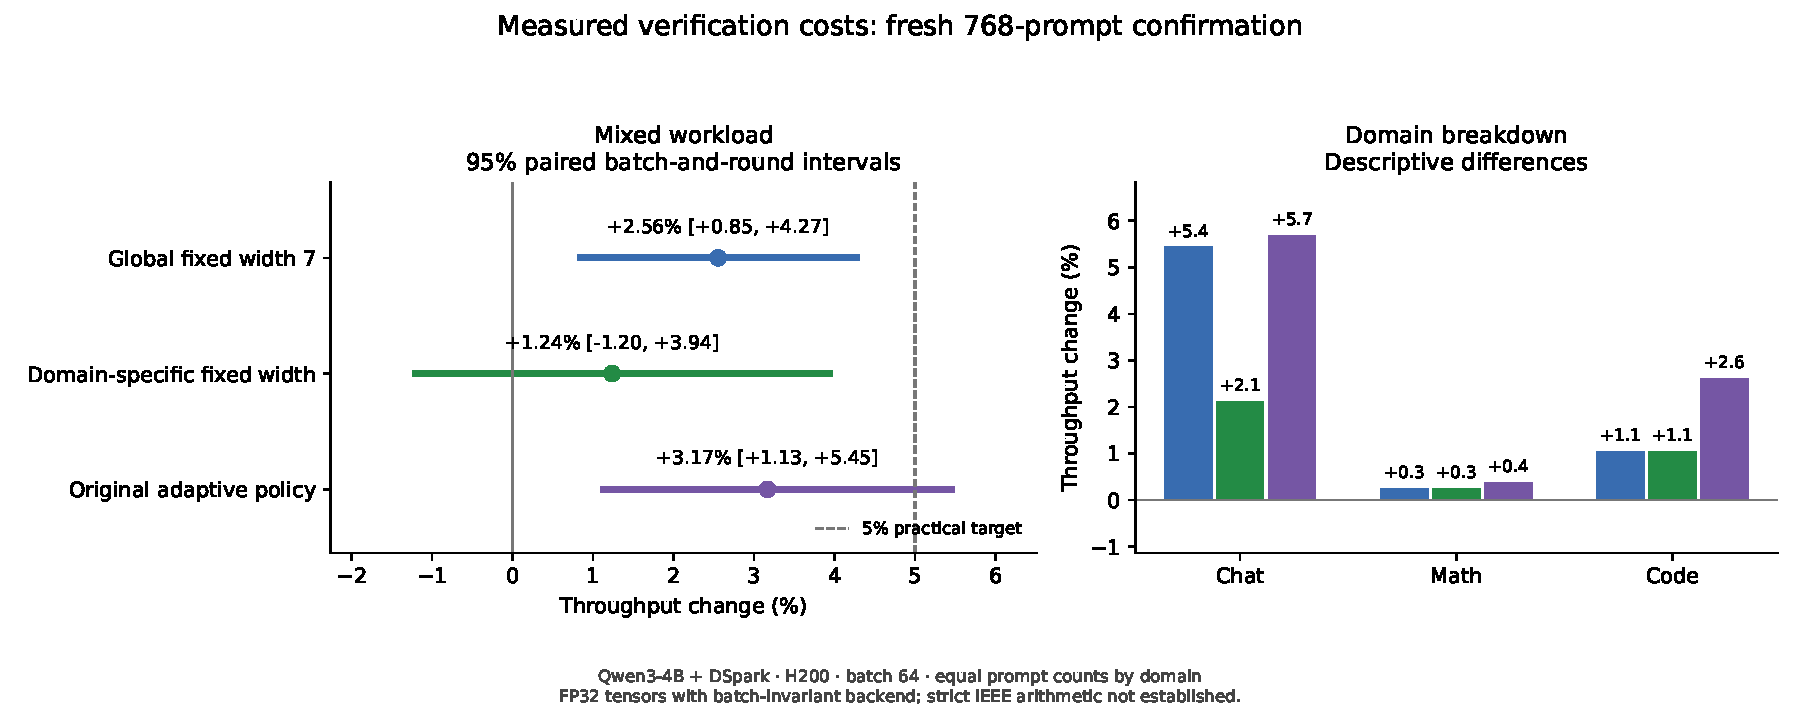
\includegraphics[width=\linewidth]{batch64_throughput.pdf}
\caption{Held-out batch-64 results. Left: aggregate gains and paired bootstrap intervals. Right: descriptive domain differences. Chat shows the largest gain against native adaptive verification.}\label{fig:confirm}
\end{figure}
\small\section{Where the result holds}
The native comparison isolates the cost estimator because both arms use the same adaptive scheduler. Beating the global fixed width at two batch sizes provides a second check that timing-aware decisions can add value on a mixed workload. The domain-specific comparison is harder: knowing the domain in advance recovers much of the advantage, and the remaining interval includes zero.

A separate exploratory batch-128 sweep on 384 reused prompts found a 2.09\% gain over native adaptive verification and a 4.10\% loss to the best fixed width (3). Its engine order was unbalanced. It identifies a regime worth testing and limits generalization from batches 32 and 64. A separate batch-64 calibration pilot also found online confidence refitting 0.24\% slower than frozen calibration. The confirmed gain comes from the cost-table intervention.

\paragraph{Mechanism and generalization.} The illustrative calculation shows how changing costs can change verification budgets. Establishing which dips produced the held-out gain requires recording disagreements on identical scheduler states and timing the alternative budgets at those states. Repeated profiles on independent engine launches could also distinguish stable decreases from noise. One natural extension would retain a decrease only when it recurs across profiles, measuring the extra profiling cost alongside steady-state throughput. Replication on a second model or accelerator would test portability.

\paragraph{Conclusion.} A running maximum over GPU timing measurements can discard information useful for speculative verification. In this deployment, retaining measured costs increased warmed-up throughput on held-out mixed workloads at two batch sizes while preserving the observed token outputs. The strongest baseline comparison and the batch-128 screen show why both the workload and the alternative policy belong in the speedup claim.

\small
\noindent\href{https://github.com/angelinaquan/adaptive-verification-for-speculative-decoding}{Code, frozen plans, and records}
\quad\href{https://wandb.ai/aquan-world-model/18657-speculative-pilot/runs/vxw4i4v4}{Batch-32 audit}
\quad\href{https://wandb.ai/aquan-world-model/18657-speculative-pilot/runs/az4k5l1i}{Batch-64 audit}
\footnotesize\begin{thebibliography}{3}\setlength{\itemsep}{0pt}
\bibitem{leviathan} Y. Leviathan, M. Kalman, and Y. Matias. \href{https://proceedings.mlr.press/v202/leviathan23a.html}{Fast Inference from Transformers via Speculative Decoding}. ICML, 2023.
\bibitem{dspark} X. Cheng et al. \href{https://arxiv.org/abs/2607.05147}{DSpark: Confidence-Scheduled Speculative Decoding with Semi-Autoregressive Generation}. 2026.
\bibitem{native} vLLM Team. \href{https://vllm.ai/blog/2026-08-14-dspark-adaptive-verification}{Adaptive Verification in vLLM}. August 2026.
\bibitem{hoeffding} W. Hoeffding. Probability inequalities for sums of bounded random variables. Journal of the American Statistical Association, 58(301), 13--30, 1963.
\end{thebibliography}
\end{document}
